\documentclass[12pt,a4paper]{report}
\usepackage{graphicx}
\usepackage{ctex}
\usepackage{indentfirst}
\usepackage{amsmath}
\graphicspath{{chapter/}{figures/}}
\usepackage{CJK}
\begin{document}


\chapter{研究背景及意义}
高降压比DC/DC变换器在工业、汽车、电信领域得到广泛应用。随着数据中心和云计算的不断发展,对电能传输的效率等指标提出了更高要求。
在数据中心领域,流行的降压比为60V/48V/24V到5V/3.3V/1.8V。传统的降压电路无法实现如此高的降压比,寻找高降压比电路的需求促生了对新型降压电路拓扑的探究。
\chapter{研究现状及分析}
Buck电路是一种典型的DC/DC拓扑结构。Buck电路结构简单,实现成本低,在电力电子与工业领域应用广泛。但是,对于一个二级Buck电路,要提高降压比,需要MOS管承受窄导通时间带来的大电流,这就在材料上对功率开关提出了极高要求。同时,高降压比所需要的极低占空比需要更高效的PWM,实际实施困难。这些因素限制了二级Buck电路的应用。
\newline

\begin{figure}[h]
    \centering
    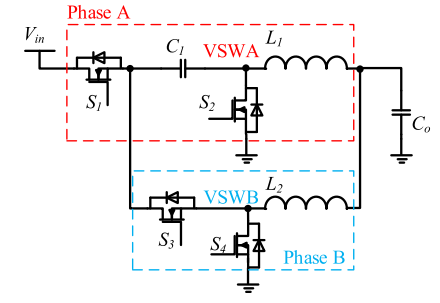
\includegraphics[width = 0.6\textwidth]{figures/SC-Buck.png}
    \caption{SC-Buck}
\end{figure}

\begin{figure}[h]
    \centering
    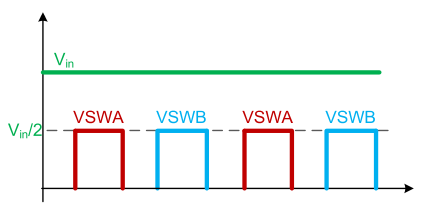
\includegraphics[width = 0.6\textwidth]{figures/SC-Buck_v.png}
    \caption{SC-Buck波形图}
\end{figure}

串联电容Buck电路(Series-capacitor Buck,SC-Buck)把开关电容和多相Buck结合到一起,形成一种新的Buck电路的拓扑结构。与传统的Buck电路相比,SC-Buck规模更小,效率更高,具有电流自平衡功能。如图2.1所示,两个电感交错放置于电路中,消除输出电容$C_o$上的电流纹波,同时还能分别减小两个电感的尺寸。图2.2表明,分到每条支路上的电压只有输入电压的一半。


实现高降压比的另一个趋势是使用磁性元件。实现方法有带倍流整流的全桥变换器(full-bridge converter with current-doubler rectifier),LLC,Sigma变换器和分接电感Buck变换器(tapped inductor Buck converter)等。在轻载时,全桥变换器无法实现所有主开关管的零电压开关(Zero-voltage Switching),导致轻载时转换效率下降,而且输出端的大电感会影响功率密度。在谐振频率下,LLC具有较高效率,但是系统不在谐振频率时的动态效率很低。为了解决这个问题,提出了将LLC和Buck结合的Sigma变换器。LLC负责谐振频率下的高效功率传输,Buck变换器负责瞬态响应。但是,由于LLC变换器在稳态时处理大部分的功率,Buck变换器在过渡时处理大部分的功率,因此LLC变换器和Buck变换器都必须设计成能够处理整个系统的功率。如此的并行结构将增大控制的复杂度。


Tapped inductor Buck转换器最初用于处理高降压比功率转换电路。然而,交错电感的漏感与开关电容产生共振,产生额外的电压环。基于混合变压器的Buck变换器(Hybrid-transformer-based Buck,HTB)增加了一个开关(S3)和一个电感,以获得软开关操作和较低的电压环,如图2.3所示。利用交错电感的漏感作为谐振电感,交错串联电容Buck(Series-capacitor tapped Buck,SC-TaB)变换器如图2.4所示。SC-TaB中的开关管$S_3$可以直接连接负载,也可以直接接地,另一种SC-TaB电路如图2.5所示。后者的两相交错配置的电路图如图2.6所示。开关管接地可以让控制更为简单。
\newline

\begin{figure}[h]
    \centering
    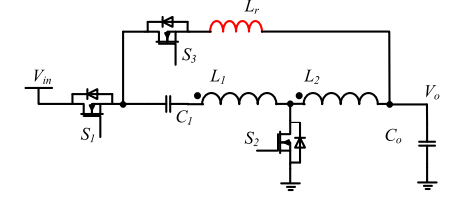
\includegraphics[width = 0.6\textwidth]{figures/HTB-Buck.png}
    \caption{HTB-Buck}
\end{figure}

\begin{figure}[h]
    \centering
    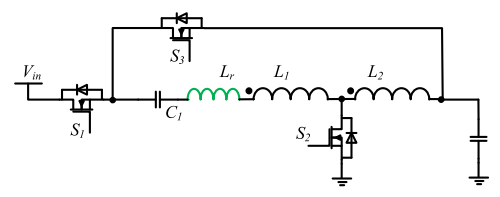
\includegraphics[width = 0.6\textwidth]{figures/SC-TaB1.png}
    \caption{SC-TaB,$S_3$接入负载}
\end{figure}

\begin{figure}[h]
    \centering
    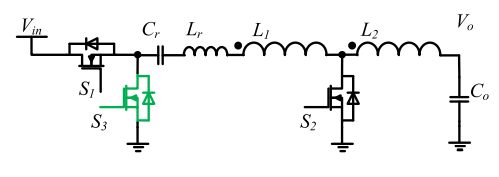
\includegraphics[width = 0.6\textwidth]{figures/SC-TaB.png}
    \caption{SC-TaB,$S_3$接地}
\end{figure}

SC-TaB和2ph-SC的主要优点是实现了所有开关管的ZVS,提高了转换效率。然而,随着降压比的增大,耦合电感的匝数比也随之增大,高匝数比会给耦合电感带来更多的应力,影响转换效率。为了克服这一缺点,并考虑到SC-Buck具有倍增降压比的能力,通过引入电容$C_1$,提出了一种新的变换器拓扑,如图2.7所示。新拓扑结构被称为交错串联电容分接Buck变换器(ISC-TaB)。该转换器将SC-Buck和SC-TaB的优点结合到一起。与传统的SC-TaB相比,它的降压比提高了一倍,使得该变换器更适合用于高降压比场合。
\newline

\begin{figure}[h]
    \centering
    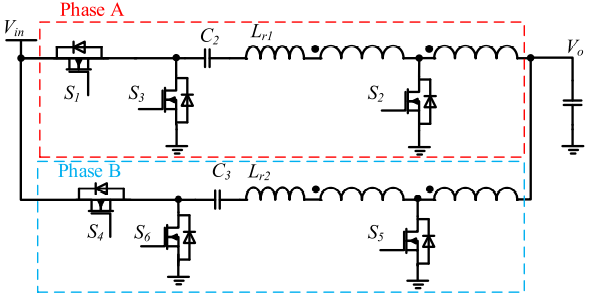
\includegraphics[width = 0.6\textwidth]{figures/2ph SC-TaB.png}
    \caption{2ph SC-TaB}
\end{figure}

\begin{figure}[h]
    \centering
    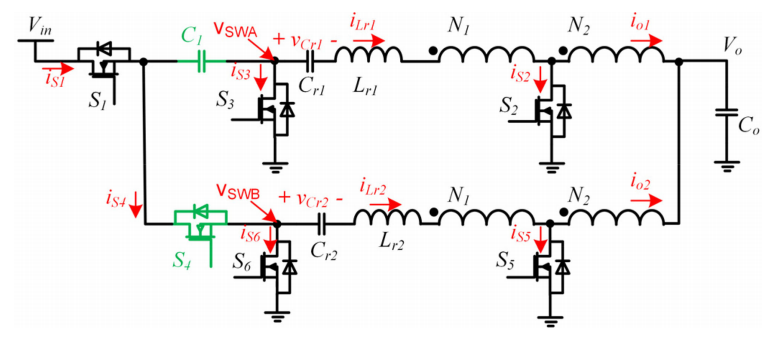
\includegraphics[width = 0.6\textwidth]{figures/circuit diagram1.png}
    \caption{ISC-TaB}
\end{figure}

\chapter{分析}
\section{运行原理}

\begin{figure}[h]
    \centering
    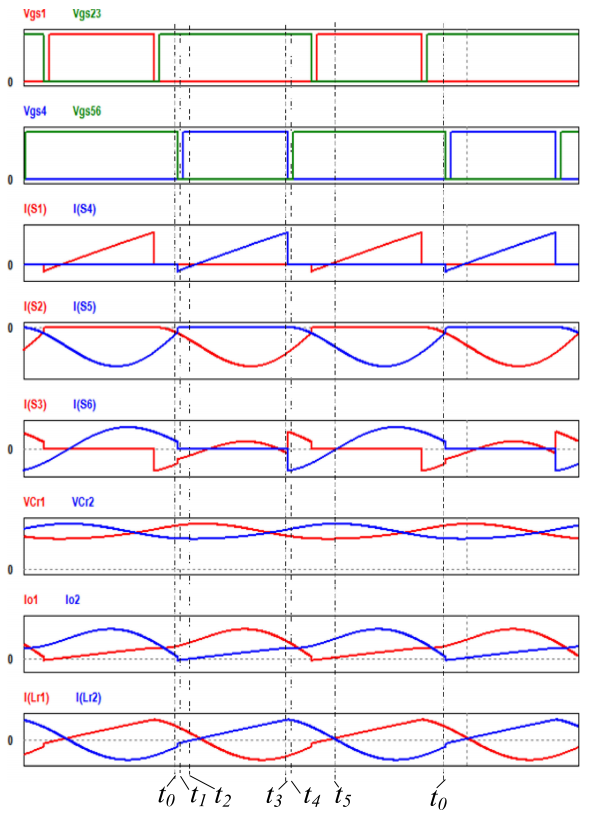
\includegraphics[width = 0.5\textwidth]{figures/waveform.png}
    \caption{ISC-TaB}
\end{figure}

\begin{figure}[h]
    \centering
    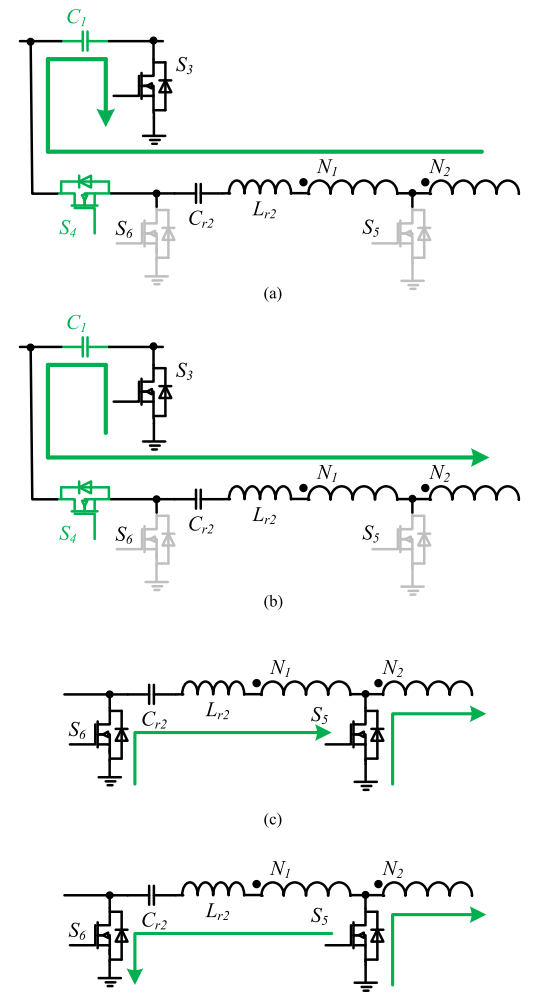
\includegraphics[width = 0.5\textwidth]{figures/current actual direction.png}
    \caption{ISC-TaB}
\end{figure}

图3.1和图3.2显示了ISC-TaB的运行机理,A相和B相原理相似。A相和B相的门控信号相差180°。
$V_{gs_1}$是$S_1$的门控信号,而$V_{gs_{23}}$是$S_2$和$S_3$的门控信号。 $V_{gs_4}$是$S_4$的门控信号,$Vgs56$是$S_5$和$S_6$的门控信号。
$I(S_1)–I(S_6)$ 分别表示电源开关$S_1-S_6$的电流。$S_2$和$S_3$同开同关。 $S_5$和$S_6$同开同关。另外,谐振电容器$C_{r_1}$和$C_{r_2}$的电压,谐振电感器$L{r_1}$和$L_{r_2}$的电流的在每个阶段的波形如图3.1所示。
在图3.2中,以B相为例说明运行机理,A相和B相的区别也将会说明。
 
$[t_0–t_2]$:此时间间隔内电流流向如图3.2(a)所示。在此时间间隔内,$iL_{r_1}$的值为负。 在$[t_0–t_1]$期间,电流流经$S_4$,为$S_4$准备零电压导通。
在$t_1$时,$S_4$零电压导通。 如图3.3中,流过励磁电感$L_m$的电流为$\left(\frac{1}{n}+1\right) i_{L r 2}$,因此耦合电感两端的电压为$\left(\frac{1}{n}+1\right)^{2} i_{L r 2} L_{m}$,在此时间间隔$[t_0–t_2]$中,$C_{r_2}$ 与$\left(\frac{1}{n}+1\right)^{2} L_{m}+L_{r 2}$ 电感谐振,在稳定状态下,$C_1$上的电压平均值为$\frac{V_{i n}}{2}$。 


可以得出谐振网络的微分方程为
\begin{equation}
    \left\{\begin{array}{l}
    \frac{V_{\mathrm{in}}}{2}-V_{o}-v_{\mathrm{Cr} 2}=L_{r 2} \frac{d i_{\mathrm{Lr} 2}}{d t}+L_{m} \frac{d i_{\mathrm{Lr} 2}}{d t} \frac{(n+1)^{2}}{n^{2}} \\
    i_{\mathrm{Lr} 2}=C_{r 2} \frac{d v_{\mathrm{Cr} 2}}{d t}
    \end{array}\right.
\end{equation}

$[t_2-t_3]$:在此时间间隔内,$C_{r_2}$持续与$(1/n+1)^2 L_m+L_r2$谐振,在$t_2$时,实际电流方向如图6(b)所示发生变化。
$[t_3-t_5]$:在时刻$t_3$,$S_4$被关闭。 在$[t_3-t_4]$期间,电流流经$S_5$和$S_6$的体二极管,$S_5$和$S_6$准备零电压导通。 电流方向如图3.2(d)所示。 在$t_4$,$S_5$和$S_6$同时开启。谐振网络由$C_{r_2}$和$L_{r_2}$组成,如图3.4所示。$[t_3-t_5]$期间的微分方程可以通过如下式子表示

\begin{equation}
    \left\{\begin{array}{l}
    -v_{\mathrm{Cr} 2}+n V_{o}=L_{r 2} \frac{d i_{\mathrm{Lr} 2}}{d t} \\
    i_{\mathrm{Lr} 2}=C_{r 2} \frac{d v_{\mathrm{Cr} 2}}{d t}
    \end{array}\right.
\end{equation}

$[t_5-t_0]$:$C_{r_2}$与$L_{r_2}$保持谐振。 在$t_5$时刻,流过谐振电感器的电流会改变其方向。 电流路径和方向如图3.2(d)所示。 在$t_0$时$S_5$和$S_6$同时关闭。 由于$i_{L_{r_2}}$的方向,电流将流过$S_4$,为下一个开关周期准备零电压导通。A相的运行与B相类似。
在$[t_0–t_3]$期间,注意到A相和B相之间的相位差, 每相都有电流流过$S_3$,这会导致$S_3$上的电流波形不同于$S_6$上的电流波形。其中的差异可见于图3.1。
\newline

\begin{figure}[h]
    \centering
    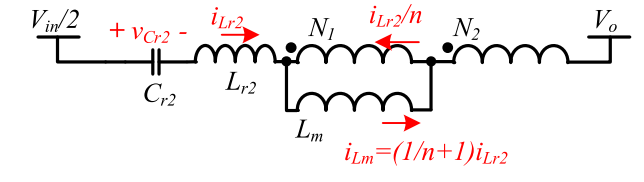
\includegraphics[width = 0.6\textwidth]{figures/current value in t0-t2.png}
    \caption{ISC-TaB}
\end{figure}

\begin{figure}[h]
    \centering
    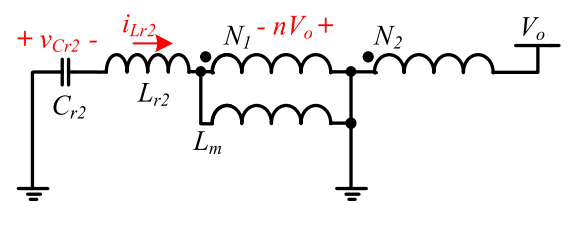
\includegraphics[width = 0.6\textwidth]{figures/current value in t3-t5.png}
    \caption{ISC-TaB}
\end{figure}

\section{降压比}
为了简化分析,使用$V_{c_{r_2}}$来表示开关周期内$C_{r_2}$上的平均电压。
$T_s$是开关周期,$DT_s$表示从$t_0$到$t_3$的时间。
根据(3.3),在$[t_0,t_3]$期间,$L_{r_2}$两端的平均电压为:
 
\begin{equation}
    V_{\mathrm{Lr} 2}=\frac{\frac{V_{\mathrm{in}}}{2}-V_{o}-V_{\mathrm{Cr} 2}}{1+\frac{L_{m}}{L_{r 2}} \cdot \frac{(n+1)^{2}}{n^{2}}}
\end{equation}

根据图7所示的电流关系,$L_m$上的电压在$[t_0,t_3]$期间为:

\begin{equation}
    V_{\mathrm{Lm}}=\frac{L_{m}}{L_{r 2}} \cdot\left(1+\frac{1}{n}\right) \cdot V_{\mathrm{Lr} 2}
\end{equation}

考虑到(3.1)和(3.2),$L_{r_2}$上的伏秒平衡关系为:

\begin{equation}
    V_{\mathrm{Lr} 2} \cdot D+\left(-V_{\mathrm{Cr} 2}+n V_{o}\right) \cdot(1-D)=0
\end{equation}

$L_{m}$上的伏秒平衡关系也可写为为:

\begin{equation}
    V_{\mathrm{Lm}} \cdot D+(1-D)\left(-n V_{o}\right)=0
\end{equation}

整合公式(3.3)到(3.6),并假设$L_{r_1}=L_{r_2}=L_{r}$,则ISC-TaB电路的降压比为:

\begin{equation}
    \frac{V_{o}}{V_{\mathrm{in}}}=\frac{D}{2 \cdot\left(n+1+\frac{L_{r}}{L_{m}} \cdot \frac{n^{2}}{n+1}\right)}
\end{equation}

Buck,SC-Buck,SC-TaB和ISC-TaB的电压转换关系图已经绘制在图9中。如(3.7)和图9所示,
建议的ISC-TaB转换器的转换比为SC-TaB的一半。 如前所述,当前提出的的ISC-TaB是一种适用于高降压DC/DC应用的拓扑。

\section{波形推导}

$S_1$和$S_4$的电流波形可以基于输入给出。 $i_{S_4}$的派生变形将在本节中以示例的方式给出。 $P_{in}$代表当前电路的总输入功率。 $I_{S4-avg}$则是 $I_{S4}$的平均值:

\begin{equation}
    I_{S4_{avg}} = \frac{P_{in}/2}{V_{in}/2}
\end{equation}

为了获得$i_{S_4}$的最小值,$L_{r_2}$的电流在$[t_0,t_3]$假设是线性的。那么$i_{S4}$的最小值可由以下关系推导

\begin{equation}
    i_{S4_{min}} =I_{S4_{avg}}-\frac{D T_{s}}{2} \cdot \frac{V_{\mathrm{Lr} 2}}{L_{r}}
\end{equation}

%%%% 不同时间段的微分方程求解
$[t_0,t_3]$:假定在$t_0$处$C_{r_2}$上的电压为$v_{C_{r_0}}$。 $t_0$处的$L_{r_2}$电流等于$i_{S_4\_min}$.$C_{r_1} = C_{r_2} = C_r$。 可以解出(3.1)中的微分方程:

\begin{equation}
    \left\{\begin{aligned}
         & v_{\mathrm{Cr} 2-D}(t)=\frac{i_{S 4-\min }}{C_{r} \omega_{1}} \sin \omega_{1} t+\left(v_{\mathrm{Cr} 0}-\left(\frac{V_{\mathrm{in}}}{2}-V_{o}\right)\right) \cos \omega_{1} t+\frac{V_{\mathrm{in}}}{2}-V_{o} \\
         & i_{\mathrm{Lr} 2-D}(t)=-C_{r} \omega_{1}\left(v_{\mathrm{Cr} 0}-\left(\frac{V_{\mathrm{in}}}{2}-V_{o}\right)\right) \sin \omega_{1} t +i_{S 4-\min } \cos \omega_{1} t
    \end{aligned}
    \right.
\end{equation}

其中$\omega_{1}=\frac{1}{\sqrt{\left[\left(\frac{1}{n}+1\right)^{2} L_{m}+L_{r}\right] \cdot C_{r}}}$

之后是$[t_3,t_0]$过程,上一个过程的结束正好是下一个过程的开始。由此求得这一段的微分方程的解:

\begin{equation}
    \left\{\begin{aligned}
        v_{\mathrm{Cr} 2-D^{\prime}}(t)=\frac{i_{\mathrm{Lr} 2-D}\left(D T_{s}\right)}{C_{r} \omega_{2}} \sin \omega_{2} t+\left(v_{\mathrm{Cr} 2-D}\left(D T_{s}\right)-n V_{o}\right)\times \cos \omega_{2} t+n V_{o} \\
        i_{\mathrm{Lr} 2-D^{\prime}}(t)=-\left.C_{r} \omega_{2}\left(v_{\mathrm{Cr} 2-D}\left(D T_{s}\right)-n V_{o}\right)\right) \sin \omega_{2} t+i_{\mathrm{Lr} 2-D}\left(D T_{s}\right) \cos \omega_{2} t
    \end{aligned}\right.
\end{equation}

其中$\omega_{1}=\frac{1}{\sqrt{L_r\cdot C_{r}}}$

在稳定状态下,$v_{C_{r_0}}$的值在切换周期开始$t_0$时刻与切换周期终点时相同。 为了求解$v_{C_{r_0}}$,可以使用以下公式:

\begin{equation}
    v_{\mathrm{Cr} 2_{-} D^{\prime}}\left((1-D) T_{s}\right)=v_{\mathrm{Cr} 0}
\end{equation}

在(3.10)中,获得$L_{r_2}$的电流波形。 基于(3.10)以及(3.4)和(3.6),可以获得励磁电流$i_{L_m}$:

\begin{equation}
    i_{\mathrm{Lm}}(t)=\left\{\begin{array}{c}
        \left(1+\frac{1}{n}\right) i_{\mathrm{Lr} 2_{-} D}(t), 0<t<D T_{s}                                                 \\
        \left(1+\frac{1}{n}\right) i_{\mathrm{Lr} 2_{-} D}\left(D T_{s}\right)-\frac{n V_{o}}{L_{m}}\left(t-D T_{s}\right) \\
        D T_{s} \leq t \leq T_{s}
    \end{array}\right.
\end{equation}

其他波形,例如流经所有开关的电流和输出电流,可以根据这些推导得出波形。根据这些导出的波形,
每个电源开关和电感绕组的均方根电流的波形可以获得,同时可以得到谐振电容器的额定电压波形。 推导波形如图10所示。
这些图表在下面的图4.1中,并附有参数。 

\section{ZVS过程详解}

结合(3.10)和(3.11),流经谐振电感的电流可以解出。
为了确保S1和S4的ZVS操作具有不同的输入电压和不同的负载电流,
当$S_3$或$S_6$关断,$i_{Lr1}$和$i_{Lr2}$的值应足够负。

为了更好地理解ZVS,当$S_3$关闭并且$S_1$将要打开时的等效电路如图11所示。
此时,$S_2$和$S_6$打开,因此它们在等效电路中直接接地。后$S_3$关断,$L_{r1}$上的剩余电流将为$C_{ds3}$和$C_{ds4}$充电.同时$C_{ds1}$放电。
在这段时间内,可以得到以下微分方程:

\begin{equation}
    \left\{\begin{array}{c}
        C_{\mathrm{ds} 1} \frac{d\left(V_{\mathrm{in}}-v_{C 1}-v_{\mathrm{SWA}}\right)}{d t}-i_{\mathrm{Lr} 1} \\
        =\left(C_{\mathrm{ds} 3}+C_{\mathrm{ds} 4}\right) \frac{d V_{\mathrm{SWA}}}{d t}                       \\
        L_{r 1} \frac{d i_{\mathrm{Lr} 1}}{d t}=v_{\mathrm{SWA}}-v_{\mathrm{Cr} 1}-V_{\mathrm{Pr} i}
    \end{array}\right.
\end{equation}

其中,初始条件为:$i_{\mathrm{Lr} 1}(0)=I_{\mathrm{Lr} 1\_0}, v_{\mathrm{SWA}}(0)=0$,其中$i_{\mathrm{Lr} 1}(0)=I_{\mathrm{Lr} 1\_0}$的值可由公式(11)求得。

为了简化分析,在ZVS过渡期间,可以将$v_{C_{r_1}}$和$v_{C_1}$视为恒定,并假定$v_{Cr1}$ = $v_{Cr0}$和$v_{C1}$ = $v_{in}/2$。 可以基于匝数比和输出电压获得$V_{pri}$,因此$V_{pri}$ = -n$V_{o}$。 然后可以求解微分方程

\begin{equation}
    \begin{aligned}
        v_{\mathrm{SWA}}(t)= & -\left(v_{\mathrm{cr} 0}-n V_{o}\right) \cos \omega_{z} t                                                                                                 \\
                             & -\frac{I_{\mathrm{Lr} 1_{-} 0}}{\omega_{z}\left(C_{\mathrm{ds} 1}+C_{\mathrm{ds} 3}+C_{\mathrm{ds} 4}\right)} \sin \omega_{z} t+v_{\mathrm{cr} 0}-n V_{o}
    \end{aligned}
\end{equation}

\begin{equation}
    \omega_{z}=\frac{1}{\sqrt{L_{r 1}\left(C_{\mathrm{ds} 1}+C_{\mathrm{ds} 3}+C_{\mathrm{ds} 4}\right)}}
\end{equation}

为了确保$S_1$的零电压导通,当$S_1$接通时,$v_{SWA}(t)$必须处于$v_{in}/2$。
如果未实现ZVS,则必须调整谐振网络以降低$I_{L_{r_{1_0}}}$。 同时,如果$I_{L_{r_{1_0}}}$太负,则会引入更多的传导损耗,因此$I_{L_{r_{1_0}}}$需要更多的优化设计。

\section{拓扑比较}
下图比较了各个拓扑网络的组成。

\begin{figure}[h]
    \centering
    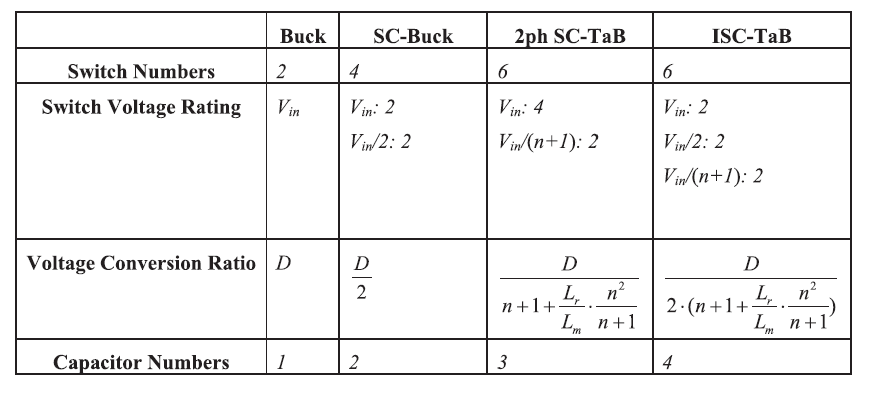
\includegraphics[width = 0.8\textwidth]{figures/table_summary.png}
    \caption{SC-TaB}
\end{figure}

\chapter{仿真电路及波形截图}
\section{仿真电路}
利用PSIM软件进行电路的仿真,参照的仿真所用的参数如图3.1所示,仿真电路图如图3.2所示。
\begin{figure}[h]
    \centering
    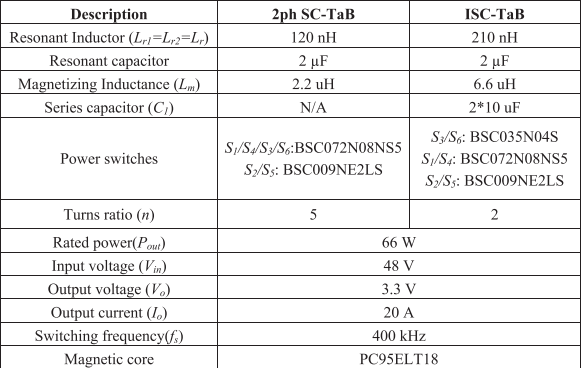
\includegraphics[width = 0.8\textwidth]{figures/parameter_table figure.png}
    \caption{元件参数表}
\end{figure}
\begin{figure}[h]
    \centering
    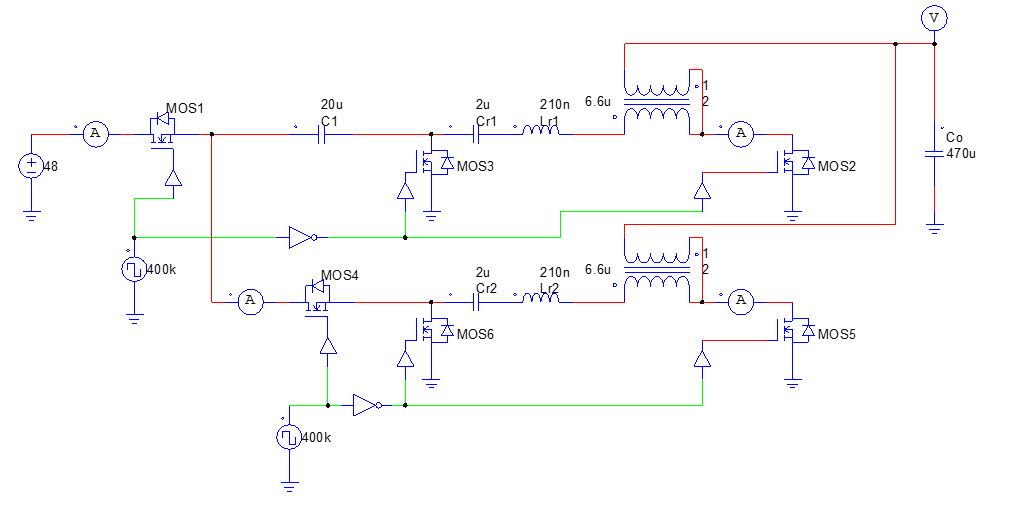
\includegraphics[width = 0.8\textwidth]{figures/PSIM-circuit diagram1.png}
    \caption{仿真电路图}
\end{figure}

实验部分波形的仿真图像如图3.3--3.7所示

输出电压稳态幅值为3.32V,误差为$0.6\%$。

\begin{figure}[h]
    \centering
    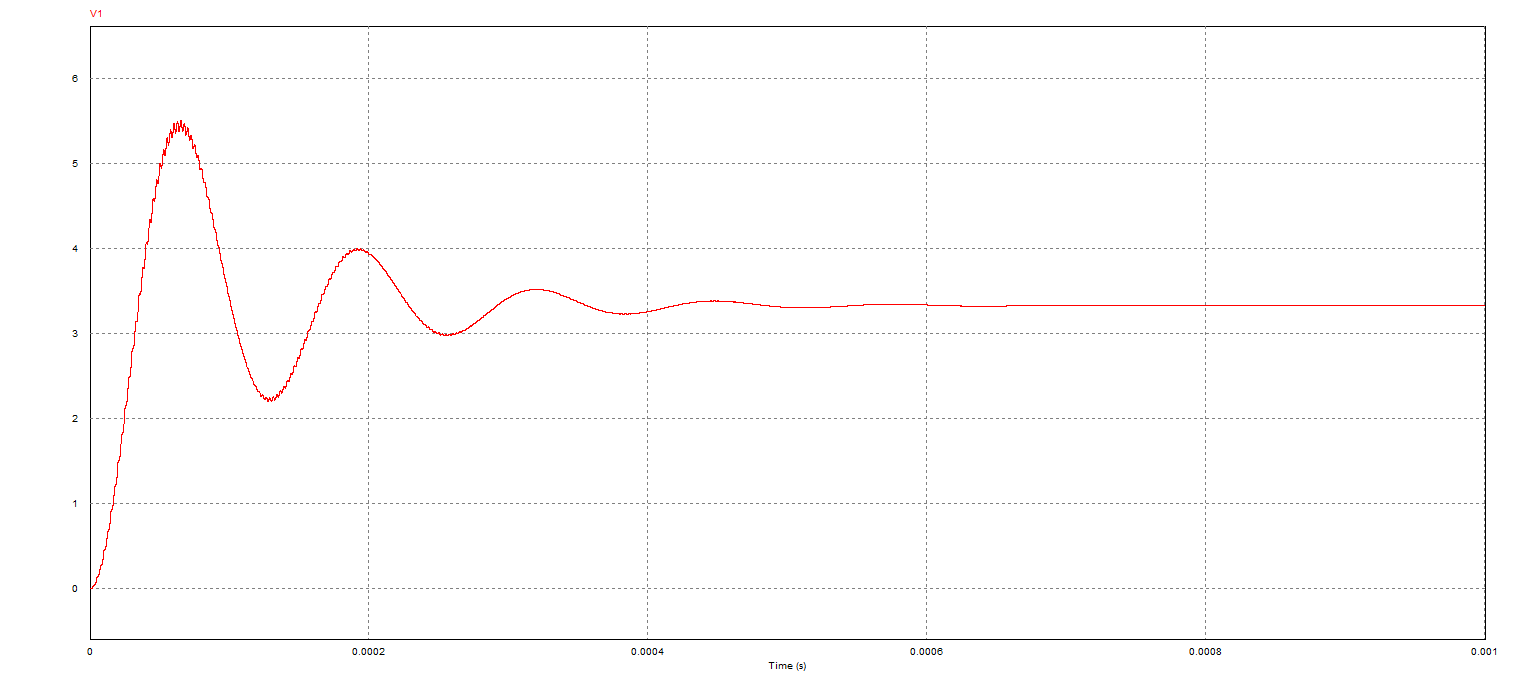
\includegraphics[width = 0.8\textwidth]{figures/sim_v_out.png}
    \caption{输出电压波形}
\end{figure}

\begin{figure}[h]
    \centering
    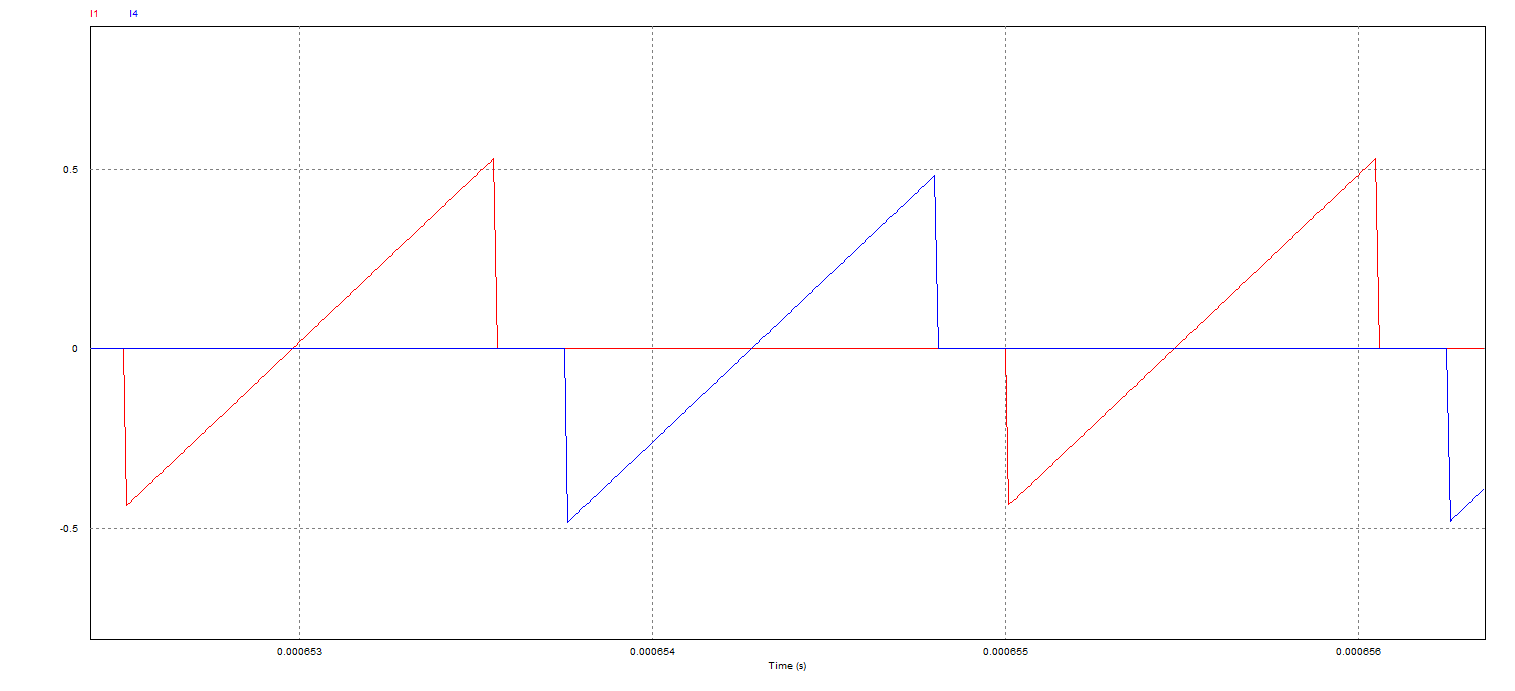
\includegraphics[width = 0.8\textwidth]{figures/sim_is1,is4.png}
    \caption{$I_{S_1},I_{S_4}$波形}
\end{figure}

\begin{figure}[h]
    \centering
    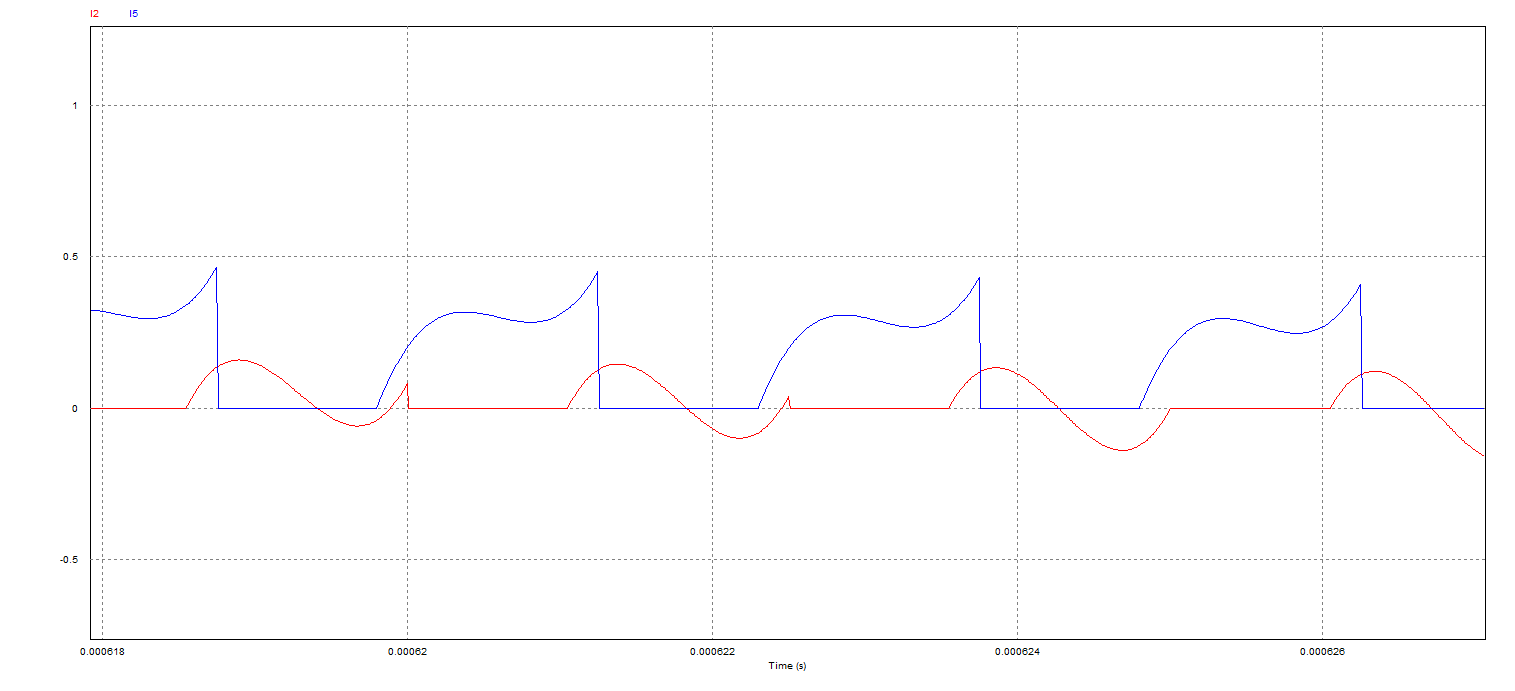
\includegraphics[width = 0.8\textwidth]{figures/sim_is2,is5.png}
    \caption{$I_{S_2},I_{S_5}$波形}
\end{figure}

\begin{figure}[h]
    \centering
    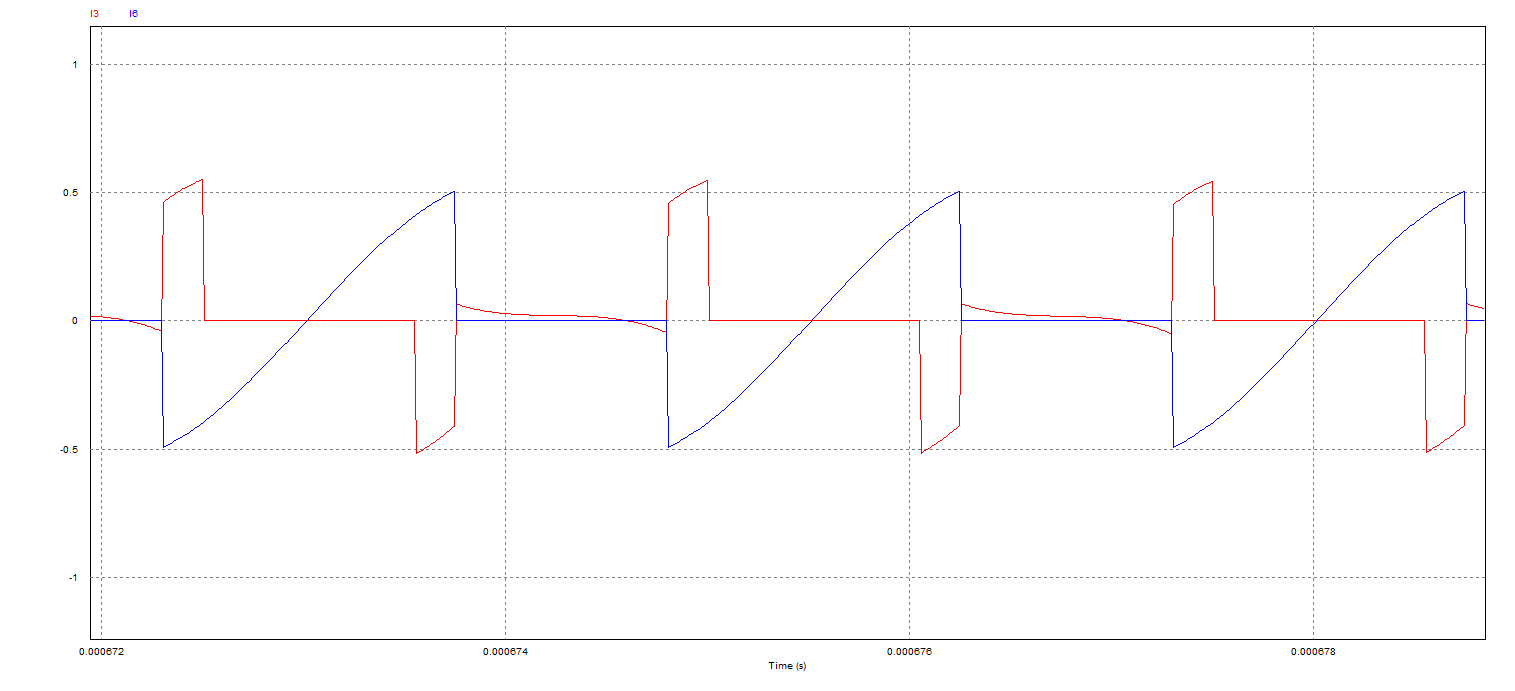
\includegraphics[width = 0.8\textwidth]{figures/sim_is3,is6.png}
    \caption{$I_{S_3},I_{S_6}$波形}
\end{figure}

\begin{figure}[h]
    \centering
    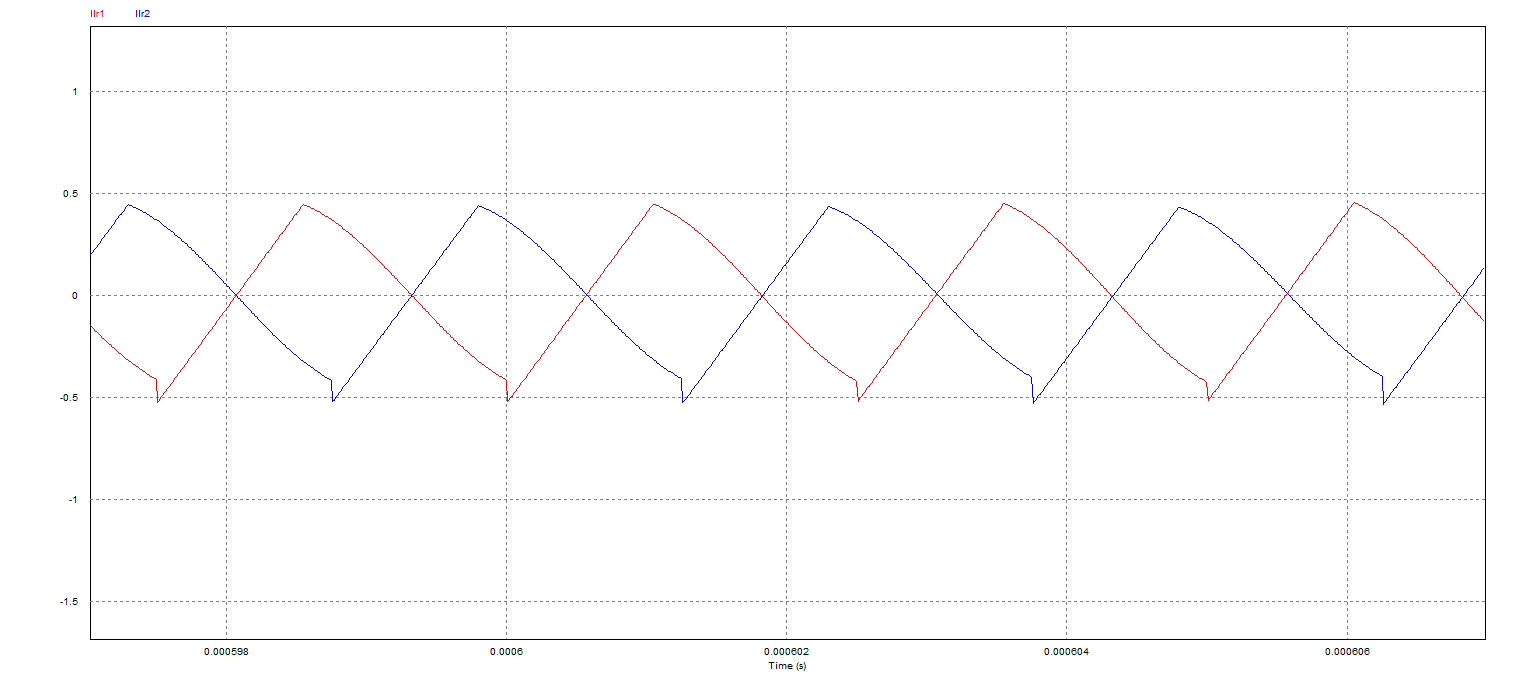
\includegraphics[width = 0.8\textwidth]{figures/sim_ilr1,ilr2.png}
    \caption{$I_{L_r1},I_{L_r2}$波形}
\end{figure}

\chapter{研究结论与思考}
%my part
本文介绍了高降压DC / DC转换器的拓扑,讨论并提出了一种新的转换器拓扑ISC-TaB转换器,并进行了分析和验证。本文的主要功能包括:

1)提出的ISC-TaB转换器结合了SC-Buck转换器和SC-TaB转换器的优势。新的拓扑结构允许S3 / S6使用低压额定功率开关和零电压导通以减少开关损耗。同时,ISC-TaB对耦合电感的压力较小,因为引入串联电容器C1会使降压比增加一倍。

2)分析了ISC-TaB转换器的工作原理
并获得所有电压和电流波形。因此,可以计算功耗以优化设计。分析了ZVS的运行,讨论了ZVS操作的设计准则。


\end{document}

